%!TEX root = ../thesis.tex
%*******************************************************************************
%****************************** Third Chapter **********************************
%*******************************************************************************
\chapter{Stato dell'arte}
\hspace{0,5cm}

\section{Definizione dei discorsi d'odio}
Nonostante la grande presenza di discorsi d'odio nel panorama dei social network, non è ancora presente una definizione nitida e universale che riesca a inquadrare il fenomeno entro una cornice precisa. Le diverse definizioni, di quello che è comunemente chiamato \textit{hate speech}, sono principalmente fornite da organizzazioni sovranazionali come l'Unione Europea in \cite{hatespeechEU}, da organizzazioni internazionali per le minoranze (ILGA \cite{ilga}), da documenti scientifici e dai termini e condizioni delle principali compagnie tecnologiche operanti nel settore social (Facebook, YouTube e Twitter in \cite{facebookhate,youtubehate,twitterhate}).

In \cite{survey2} viene svolto un lavoro di analisi su queste fonti e vengono sommarizzate efficacemente fornendo la seguente definizione tradotta di \textit{hate speech}:

\begin{quote}
    \textit{Il discorso d'odio è un linguaggio che attacca o sminuisce, incita violenza o odio verso dei gruppi, basandosi su specifiche caratteristiche quali l'apparenza fisica, la religione, la discendenza, la nazionalità o le origini etniche, l'orientamento sessuale, l'identità di genere o altro, e può verificarsi in diversi stili linguistici, anche in forma subdola o con l'uso di umorismo.}
\end{quote}

Su questa definizione appena introdotta si baserà il lavoro svolto per la classificazione dei contenuti d'odio online.



\section{Lavori relativi al riconoscimento dei discorsi d'odio}

Il problema di riconoscimento dei discorsi d'odio sui social network, seppur sia ancora nella sua fase iniziale, è in rapida evoluzione. Ad esempio, non è ancora presente un benchmark universale per testare le performance di una qualsiasi tecnica utilizzata e la gran parte dei testi usati per la classificazione vengono generati caso per caso, variando di molto il tipo di linguaggio utilizzato \cite{hatespeechSurvey}, tuttavia è presente un vasto numero di metodologie in grado di identificare testi offensivi e denigratori. Eccezion fatta per pochi casi (\cite{fersES,HateData1,HateData2,HateData3,HateData4}), la stragrande maggioranza di dataset rimangono spesso privati, limitando la possibilità di eventuali confronti tra diversi metodi di classificazione.
Un’ulteriore problematica presente nel settore è costituita dalla scarsa variabilità relativa ai social network utilizzati, difatti la maggior parte degli studi usa Twitter come unica piattaforma per la raccolta di informazioni. Tra le probabili cause di questo fenomeno è sicuramente presente l'oggettiva difficoltà riscontrata durante la raccolta dei dati, molte volte limitata o perfino bloccata dalle stesse piattaforme social per tutelare la privacy dei propri utenti. Esplorando la letteratura presente è inoltre evidente come la lingua più analizzata sia l’inglese, con alcune più rare eccezioni per le lingue europee più diffuse quali tedesco, spagnolo, francese e italiano, rimanendo comunque poco sufficienti a fornire un quadro chiaro della situazione dei fenomeni di odio online nei diversi paesi del mondo.

Diversi studi sono stati effettuati con lo scopo di riconoscere i diversi tipi di hate speech online classificandoli in base ai loro attributi: nella maggior parte dei casi le statistiche descrittive evidenziano una forte presenza di razzismo \cite{LocateHate}, sessismo e misoginia \cite{SarahMiso,fersES,JamieMiso}, pregiudizi contro immigrati \cite{rnnabusive} e omofobia \cite{VasuHomophobia}. Nonostante la presenza di diverse categorie però, una gran parte degli studi si concentra su una classificazione esclusivamente binaria, lasciando in sospeso ad eventuali sviluppi futuri il riconoscimento di tutte le sottocategorie precedentemente elencate.


Il riconoscimento dei discorsi d’odio online viene svolto attraverso tecniche di text mining, ovvero un'analisi del lessico utilizzato nei dati relativi alla ricerca. Generalmente vengono prese in considerazione diverse caratteristiche dei testi per trovare la/e combinazioni che permettono una migliore classificazione dei discorsi d’odio.


\subsection{Dizionari}

La strategia più semplice utilizzata per l’analisi dei testi è sicuramente l’uso dei dizionari, ossia raccolte di parole offensive e denigratorie che vengono generalmente usate in commenti contenenti discorsi d’odio. Contando il numero di occorrenze delle parole offensive o usando la normalizzazione sulla base della lunghezza del testo considerato, è possibile generare un punteggio che indichi con quanta probabilità il commento appartenga alla classe dei discorsi d’odio.

Diversi miglioramenti a questo approccio vengono evidenziati in studi \cite{WilliamHate, languagedetect,SriCyberbullying} che fanno uso della \textit{distance metric}, una tecnica in grado di mitigare il problema del mascheramento delle parole. Questa procedura, usata dagli utenti online per ingannare il riconoscimento automatico dei termini offensivi, riguarda nella maggior parte dei casi la sostituzione di un carattere all’interno di una parola pur mantenendone un aspetto visivo simile all’originale. Come esempio esplicativo, calcolando il minimo numero di modifiche da apportare la parola mascherata “\textit{stup1d0}”, è possibile associarla alla sua forma originale “\textit{stupido}”, presente in un qualsiasi dizionario come termine chiaramente offensivo.

Il confronto tra i testi esaminati e i dizionari contenenti parole offensive come \cite{Hurtlex,ShuhuaDict,KarthikDict,MaralDict} riesce nella maggior parte dei casi a individuare i commenti negativi, pur mancando ancora di precisione nella divisione delle classi e generando una grande quantità di falsi positivi. Osservando il lavoro svolto in \cite{cyberbullying} è evidente come una classificazione di questo tipo sia inefficace nel rappresentare il contesto entro il quale un determinato termine è inserito: secondo lo studio il 48\% dei testi presi in esame non rientra nella classe dei negativi nonostante contenga un’alta percentuale di parole denigratorie.

Un ulteriore supporto per la classificazione viene fornito dall'analisi di diversi fattori concorrenti ad un probabile atteggiamento denigratorio da parte di un commento \cite{Chen,offensivelang}. Osservando i riferimenti esterni come URL o hashtag è generalmente possibile attribuire un contesto entro il quale il testo in analisi è inserito o, analizzando la sua punteggiatura e la sua capitalizzazione, si è in grado costruire un pattern che caratterizza i commenti di tipo negativo.

\subsection{Bag of words e N-grams}

Tra le tecniche che più in assoluto vengono impiegate, anche per migliorare lo scarso riconoscimento del contesto da parte dei dizionari, troviamo sicuramente le raccolte di parole (o \textit{Bag-of-words}) in \cite{BOWPete,BOWGreevy,LocateHate} e le \textit{N-grams} in \cite{NgPinkesh,BOWPete,offensivelang,BOWGreevy,stem2,languagedetect,NgZeerak}: la prima consiste in un procedura in grado di creare un corpus a partire dalle parole usate nei dati in analisi ed estrarne successivamente le relative frequenze; nella seconda vengono raccolte una serie di N parole consecutive in seguito usate per l’addestramento di un modello classificatore. 
L’utilizzo di \textit{bag-of-words} dimostra però ancora una scarsa efficacia nel riconoscimento del contesto che viene parzialmente migliorata dalla tecnica \textit{N-grams}. Come messo in evidenza in \cite{BOWPete} una delle problematiche che affligge \textit{N-grams} riguarda la distanza tra le parole considerate che, se maggiore di N, influisce negativamente sull'efficacia di questa tecnica. 
Nel medesimo studio viene altresì proposta una variante della stessa tecnica che, una volta identificati i termini offensivi con l’ausilio di un dizionario, raccoglie un numero prefissato di parole nell’immediato intorno. Come evidenziato in \cite{Chen} però, il problema principale di queste metodologie è rappresentato dalla numerosità di termini nella finestra considerata: al loro aumentare corrisponde un accrescimento esponenziale della complessità di calcolo necessaria alla classificazione.

\subsection{Analisi sulla sintassi}

Grazie ai miglioramenti effettuati su modelli in grado di svolgere analisi grammaticali dei testi, è possibile usare le informazioni sintattiche per meglio comprendere come ogni termine è messo in correlazione con tutti gli altri che compongono una determinata frase (\textit{LSF} o \textit{Lexical Syntactic Feature-based}). Passi avanti in questo senso sono stati svolti da \cite{StanfordNLP}, riuscendo ad associare correttamente gli aggettivi e gli avverbi verso i soggetti a cui si riferiscono. Nello studio \cite{Chen} viene proposta una tecnica di classificazione in grado di sfruttare queste caratteristiche concentrandosi sugli aggettivi considerati come negativi rivolti verso dei soggetti esterni; i risultati dimostrano un ottimo miglioramento rispetto ai metodi di classificazione precedentemente elencati.

Ulteriori sviluppi riguardanti l'analisi della sintassi di una frase riportati nel medesimo studio riguardano la raccolta delle dipendenze tra le diverse parole utilizzate. In particolar modo vengono analizzate le coppie composte da un termine governatore e dalla sua relativa apposizione per trovare riferimenti negativi attribuiti al soggetto della frase.


\subsection{Analisi dei contenuti}

Ulteriori strategie proposte dalla comunità scientifica comprendono la possibilità di studiare non solo il comportamento di ogni termine della frase in analisi, ma anche l'argomento e il contenuto generale della stessa per aumentare la precisione nel riconoscimento dei discorsi d'odio.

L’analisi dei sentimenti, generalmente negativi in caso di hate speech, è la tecnica più utilizzata in questo senso come in \cite{agarwal2017characterizing,offensivelang,stem2,ShuhuaDict,VignaInproceedings,articleNjagi}. Metodi di classificazione di questo tipo vengono spesso usati in combinazione con altre caratteristiche come l'analisi dei soggetti di una frase. Negli studi proposti viene ad esempio dimostrato come le minoranze o le persone con delle caratteristiche specifiche, siano i soggetti più esposti al fenomeno di hate speech.

Ulteriori analisi si concentrano sugli argomenti trattati nel testo da classificare, osservando lo schieramento e la polarità di un determinato commento è possibile estrarre un'ulteriore caratteristica che aiuta nel processo di identificazione del discorso d'odio.

Insieme al riconoscimento del testo in alcuni studi vengono impiegati anche diversi elementi che concorrono contemporaneamente alla classificazione di testi denigratori. È il caso di \cite{memeAndText} dove sono state analizzate le immagini insieme alla loro descrizione usando diverse tecniche e algoritmi.

Una delle ultime tecniche di text mining usate è la misurazione dell'importanza di un termine analizzando il testo dal quale è stato estratto (\textit{TF-IDF} o \textit{Term Frequency-Inverse Document Frequency}). Osservando la frequenza con cui una parola occorre in una frase è possibile attribuire un punteggio che indichi la sua rilevanza rispetto a tutti gli altri termini presenti. Nello studio \cite{KarthikDict} viene sfruttata questa pratica dimostrando come riesca a migliorare i risultati ottenuti per la classificazione dei discorsi d'odio relativi al caso di cyberbullismo.



\subsection{Classificazione supervisionata e deep learning}

Con il passare del tempo e il conseguente aumento della potenza di calcolo, diverse tecniche più complesse sono state applicate al riconoscimento dei discorsi d’odio: l’utilizzo di modelli ad apprendimento supervisionato quali Support Vector Machine (in \cite{WilliamHate}) e Naïve Bayes (in \cite{AmirNB}), analizzando la rappresentazione vettoriale dei testi, costituivano fino a poco tempo fa lo standard per classificazioni di questo tipo \cite{survey2}.

Solo più di recente sono stati introdotti modelli basati su reti neurali profonde in grado di apprendere al meglio il contesto di una frase data in input: è il caso di \cite{rnnabusive} dove una rete neurale ricorrente è stata impiegata per il riconoscimento del testo. La caratteristica principale di questa rete è quella di “ricordare” parzialmente ciò che riceve in input, permettendo quindi una buona contestualizzazione di ogni parola nella frase che la racchiude.

Altri tentativi di classificazione sono stati effettuati con reti neurali convoluzionali (o CNN) e confrontati con le reti neurali ricorrenti: i risultati ottenuti in \cite{CNNstudy} dimostrano come, nonostante un'ottima capacità nel riconoscimento del contesto, le reti ricorrenti mantengano comunque una leggera superiorità in termini di punteggi ottenuti per il riconoscimento dell’hate speech online.

Attualmente lo stato dell’arte nella comprensione del linguaggio naturale è rappresentato dai modelli basasti su reti di tipo transformer addestrati su corpus estremamente grandi: i loro punteggi in termini di precisione superano le alternative precedenti nella maggior parte dei dati analizzati. La numerosità degli studi che sfruttano reti di tipo transformer per identificare i discorsi d’odio online è ancora bassa data la recente diffusione di questi modelli ma, per i pochi già presenti come \cite{transformer1,transformer2}, i risultati sembrano essere promettenti per questo genere di classificazione. Mancano tuttavia dei confronti che permettano di comparare le performance ottenute dai modelli di tipo transformer con altri metodi di classificazione elencati precedentemente.

Passi avanti nella ricerca e nell'ottimizzazione dei modelli di questo tipo sono stati portati avanti principalmente da Google in \cite{Attention} e da OpenAI in \cite{brown2020language}, grandi aziende e associazioni che hanno la possibilità tecnologica per poter addestrare modelli così estesi e onerosi di dati.





\section{Strumenti tecnologici utilizzati}
% citare text mining, fine tuning, huggin face, ecc
Il processo di text mining consente la trasformazione del testo non strutturato in un formato ordinato per una successiva schematizzazione e analisi della sintassi. Gli strumenti offerti da \cite{Stanza} permettono un'efficace scomposizione del testo e dei suoi contenuti, riuscendo opportunamente nella riduzione delle forme flessive o correlate di una parola alla loro forma base comune. A questo scopo esistono due principali tecniche: lo \textit{stemming}, meno complesso della \textit{lemmatizzazione} e per questo largamente più utilizzato come in \cite{stem1,offensivelang,stem2}, si riferisce ad un semplice processo euristico di troncamento dell'ultima parte della parola, auspicando di estrarre una sequenza che si avvicina il più possibile alla forma base. La lemmatizzazione è invece riferita all'analisi morfologica del termine per ottenerne, attraverso l'uso di un vocabolario, il lemma (o forma base) della parola originale.

La rappresentazione del testo è invece ben generalizzata dai modelli BERT presenti nella libreria di \cite{huggingface}. Il successivo compito di classificazione, come nel caso del riconoscimento dei discorsi d'odio, viene generalmente effettuato attraverso l'uso di tecniche di \textit{transfer learning} (o \textit{domain adaptation}): il \textit{fine tuning} è sicuramente uno tra gli approcci più diffusi considerati i suoi vantaggi in termini di risparmio di tempo e
risorse computazionali durante la fase di addestramento. Mediante il processo di fine tuning i pesi relativi alle connessioni tra i vari neuroni nei modelli vengono lievemente modificati rispetto alla loro versione originale, adattandoli ai dati presenti in input ma mantenendo comunque un tasso di apprendimento più basso rispetto alla normale fase di pre-addestramento. È ulteriormente possibile "congelare" alcuni layer e conseguentemente aggiungerne di altri di diverso tipo per provare ad ottenere diversi risultati in base alle caratteristiche degli stessi layer aggiunti.


%BERT, il modello sviluppato da Google, è attualmente l’unico open source e disponibile alla comunità scientifica.


\subsection{Il modello BERT}
    BERT, acronimo di Bidirectional Encoder Representations from Transformers \cite{Bert}, è un modello sviluppato e pre-addestrato da Google di tipo Transformer che adotta meccanismi di attenzione pesando ogni elemento fornito in input. A differenza delle reti neurali ricorrenti, largamente utilizzate nel riconoscimento del linguaggio naturale, le reti di tipo Transformer non necessitano di elaborare i dati in ordine ma riescono a fornire un contesto per ogni posizione presente nella sequenza data in input.

    \begin{figure}[h!]
        \centering
        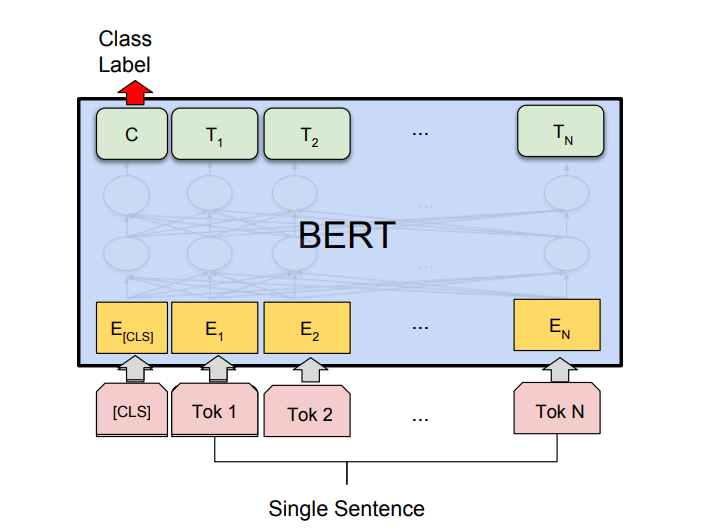
\includegraphics[width=0.5\textwidth]{pics/oth/bert for classification.png}
        \caption{Single sentence classification task, BERT}
        \label{fig:bert-classification}
    \end{figure}


    % leggere ulteriori informazioni dalle conclusioni del paper relativo a BERT (o introduzione o abstract o come vuoi insomma ciao)
    Tra i diversi impieghi del modello BERT è possibile usare il token specialce \textit{[CLS]} come illustrato in \ref{fig:bert-classification} per indicare il task di classificazione di una determinata frase. Dopo una prima fase di conversione delle parole in tokens il modello ne seleziona uno casualmente e, mascherandolo, cerca di predirlo autonomamente: questa procedura, chiamata dagli autori \textit{Masked LM}, forza la rete nel mantenere una rappresentazione del constesto distribuita su tutto il corpo della frase e non solo sui token antecedenti e successivi rispetto a quello considerato. La rappresentazione finale del testo, ottenuta leggendo gli output dell'ultimo layer del modello, permette una classificazione efficace in una delle classi che meglio descrive la frase fornita in input.
